\section{FaBoのピンの種類とケーブルの種類}
FaBoのシールドにはブリックとRaspberry Piを\ruby{繋}{つな}ぐためのピンがあります。ピンの種類には「GPIO」、「A」、「I2C」があります。下の表のように使い方が分けられているので、間違えないように気をつけましょう。\\
\begin{figure}[H]
  \begin{center}
    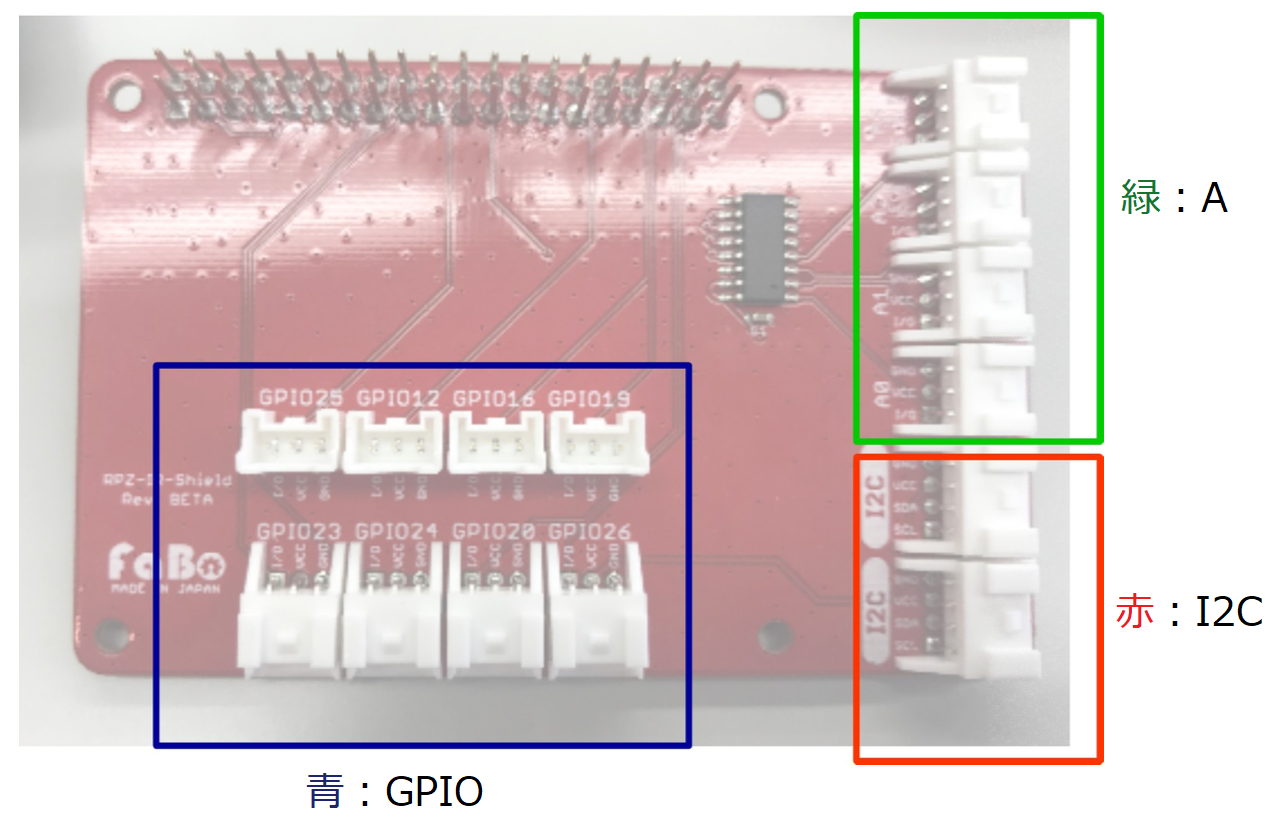
\includegraphics[width=0.5\hsize]{images/chap05/text05-img012.png}
    \caption{Faboシールドのピン配置}
  \end{center}
\end{figure}

今まで使ってきたセンサーボードでは、LEDのピンの\ruby{割}{わ}り当てがGPIO17、GPIO18、GPIO22、GPIO24となっており、あらかじめ決められた番号に割り当てられていました。しかしFaBoのGPIOはどの番号につなげても使えます。ただし、プログラムも番号に合わせて書く必要があります。\\
\begin{table}[H]
  \centering
  \caption{FaBoで使うことができるピン}
  \begin{widerrows} 
    \begin{tabular}{|c|l|} \hline
      GPIO 12 & \multirow{8}{*}{ボタンやスイッチなどのデジタル用のピン} \\ \cline{1-1}
      GPIO 16 & \\ \cline{1-1} GPIO 19 & \\ \cline{1-1} GPIO 20 & \\ \cline{1-1} GPIO 23 & \\ \cline{1-1}
      GPIO 24 & \\ \cline{1-1} GPIO 25 & \\ \cline{1-1} GPIO 26 & \\ \hline
      A0 & \multirow{4}{*}{ボリュームや\ruby{距離}{きょ|り}センサーなどのアナログ用のピン} \\ \cline{1-1}
      A1 & \\ \cline{1-1} A2 & \\ \cline{1-1} A3 & \\ \hline
      I2C & \ruby{有機}{ゆう|き}ELディスプレイのような特別な通信のためのピン \\ \hline
    \end{tabular}
  \end{widerrows} 
\end{table}

ケーブルは3ピンと4ピンの2種類があります。今回4ピンは\ruby{有機}{ゆう|き}ELディスプレイで使います。\\
% \begin{figure}[h]
%   \begin{center}
%     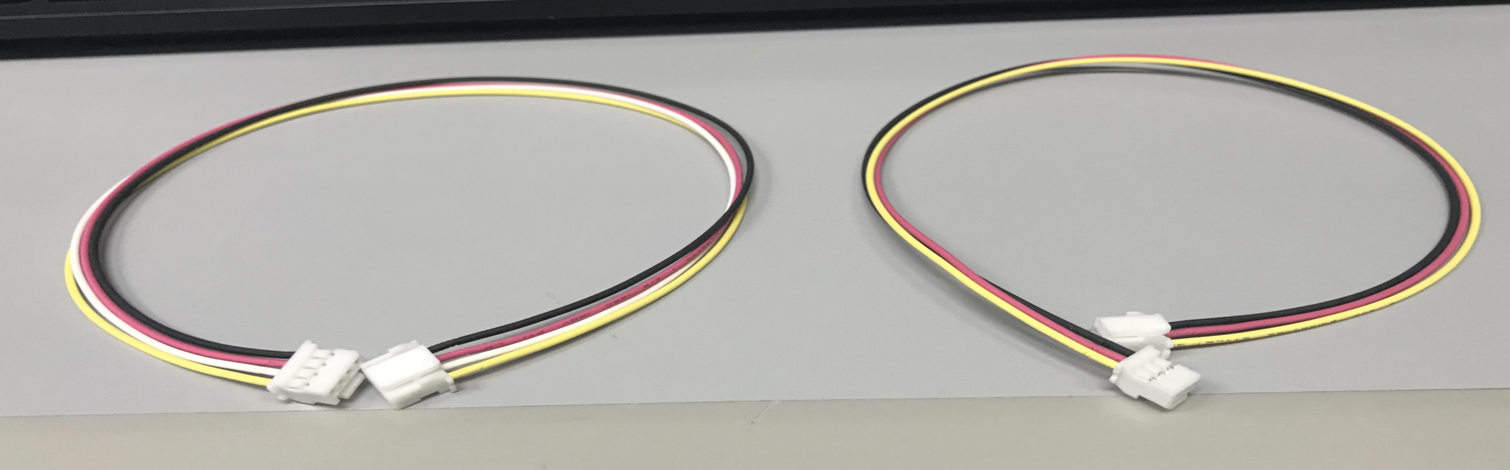
\includegraphics[scale=0.6]{images/chap05/text05-img013.png}
%     \caption{4ピンケーブルと3ピンケーブル(全体)}
%   \end{center}
% \end{figure}
\begin{figure}[H]
  \begin{minipage}[t]{0.48\columnwidth}
    \centering
    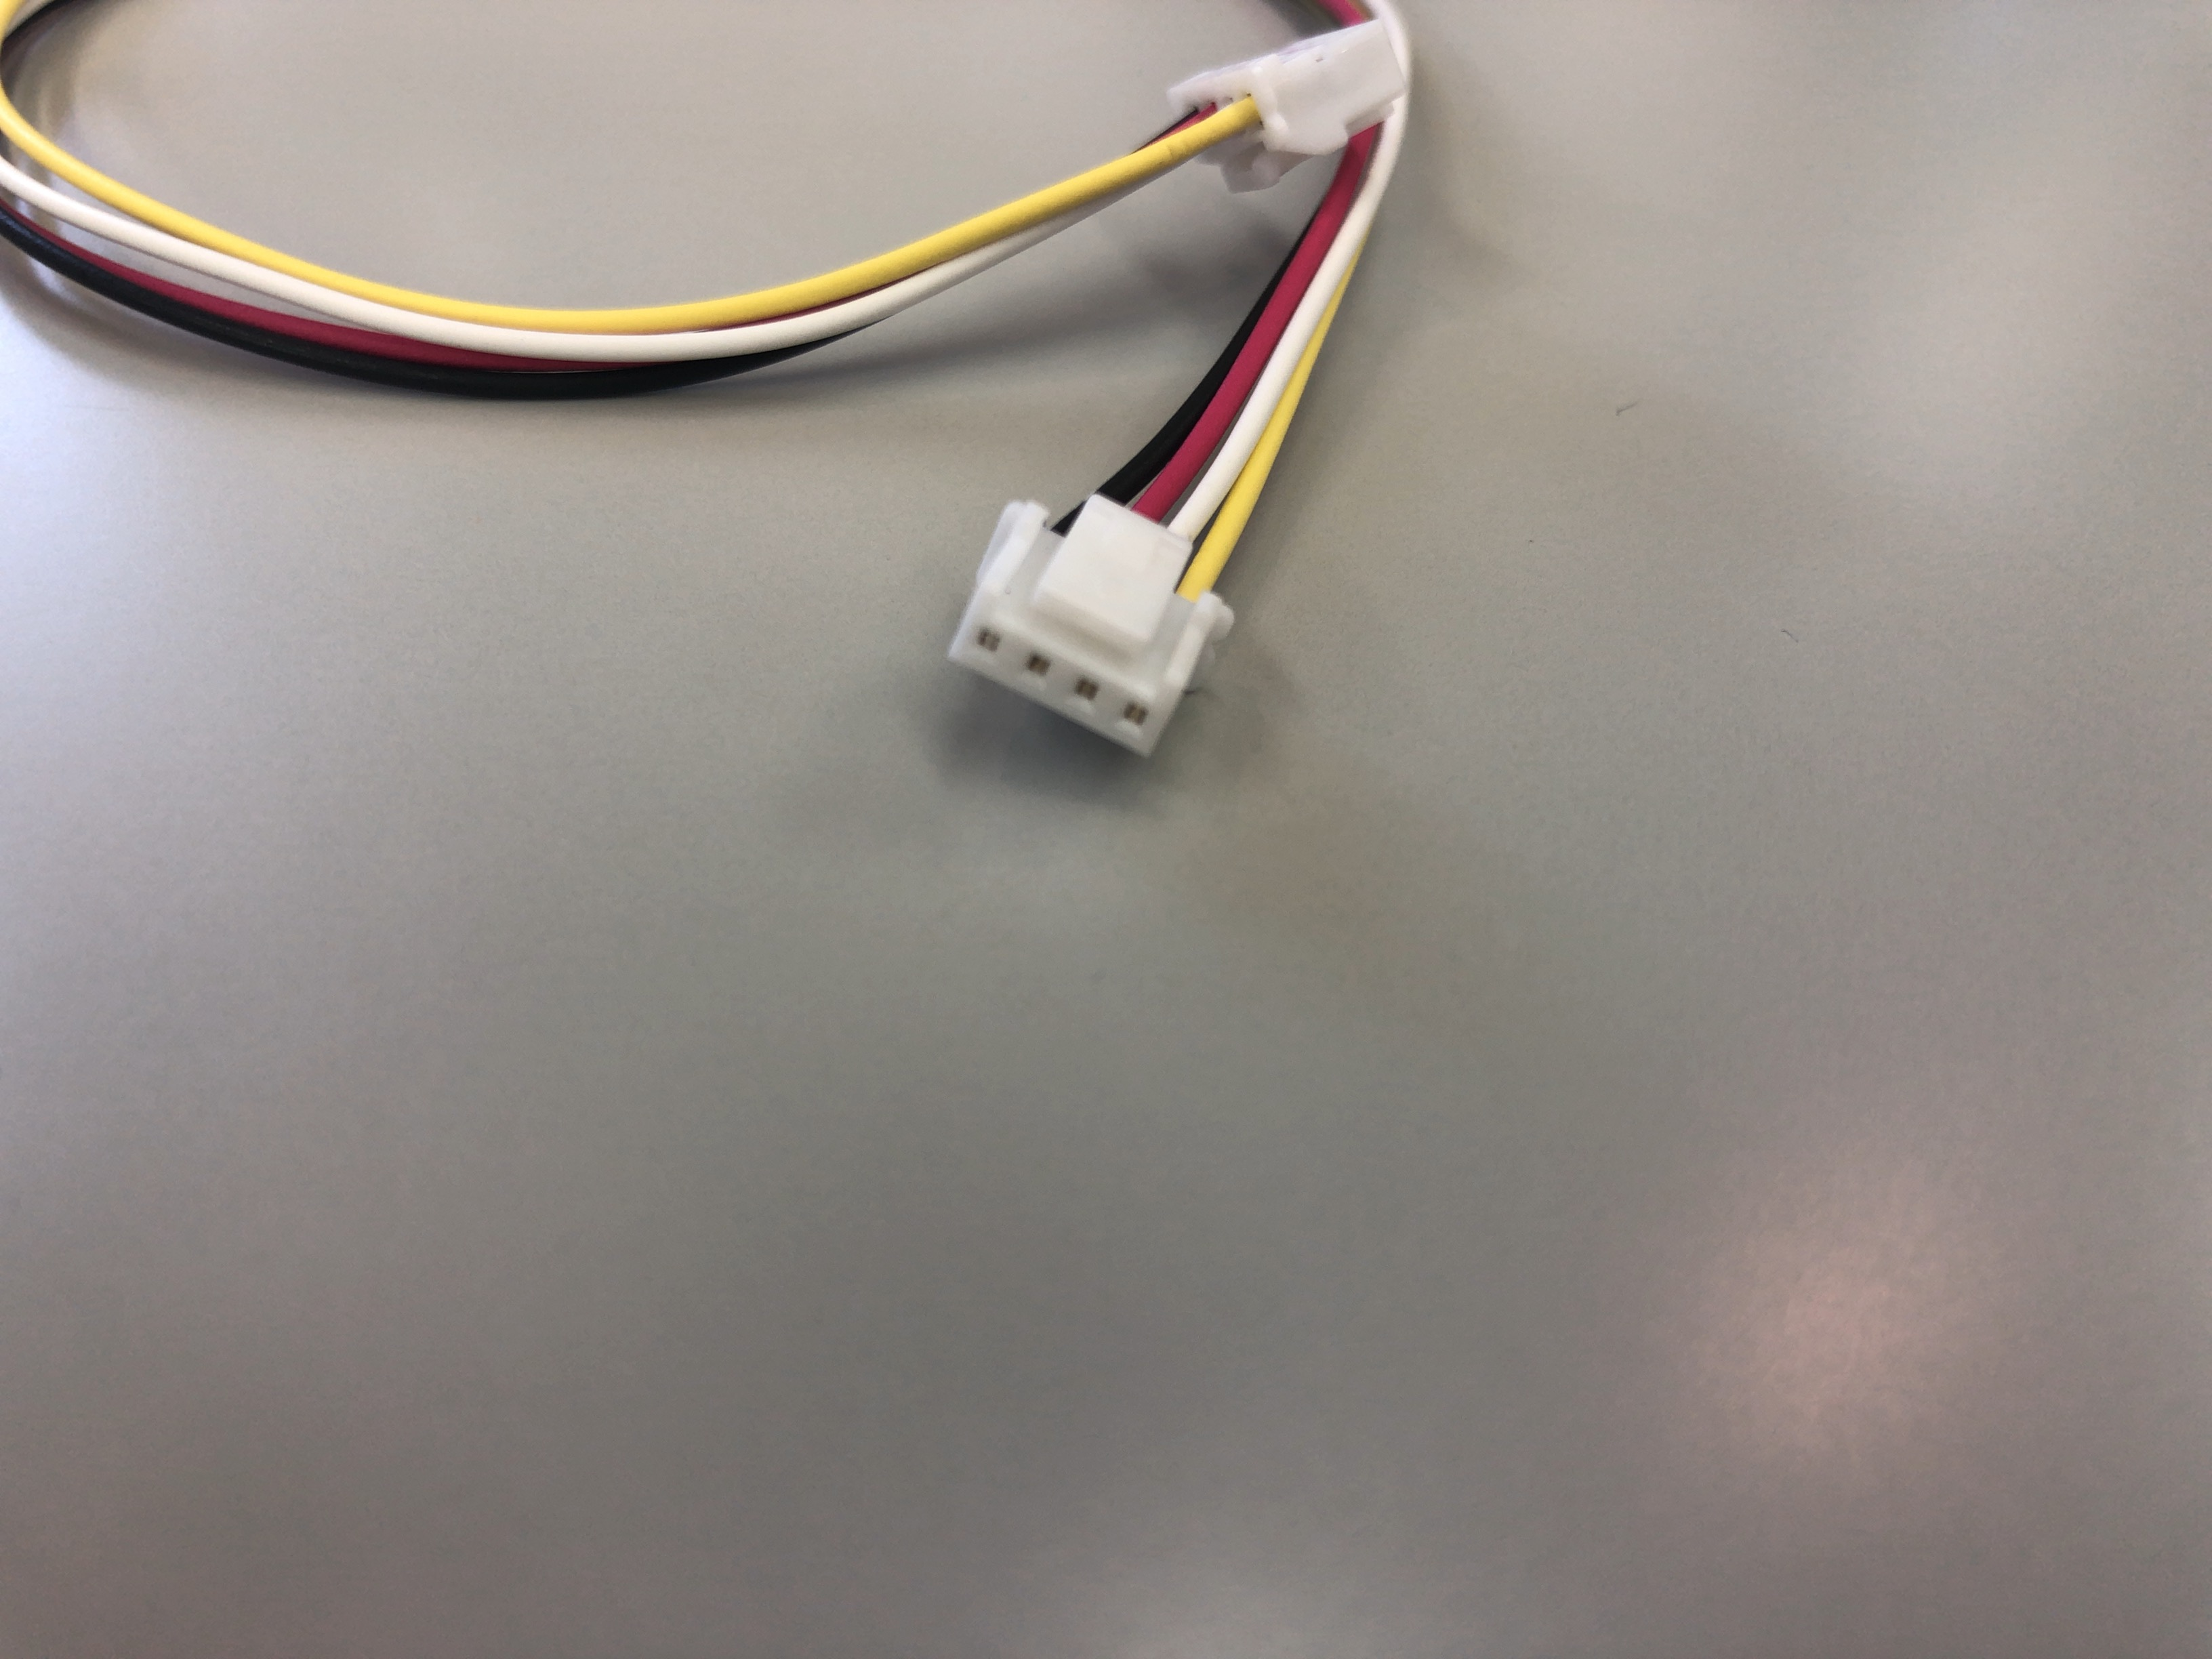
\includegraphics[width=0.8\hsize]{images/chap05/text05-img014.jpg}
    \caption{4ピンケーブル}
  \end{minipage}
  \hspace{0.04\columnwidth} % ここで隙間作成
  \begin{minipage}[t]{0.48\columnwidth}
    \centering
    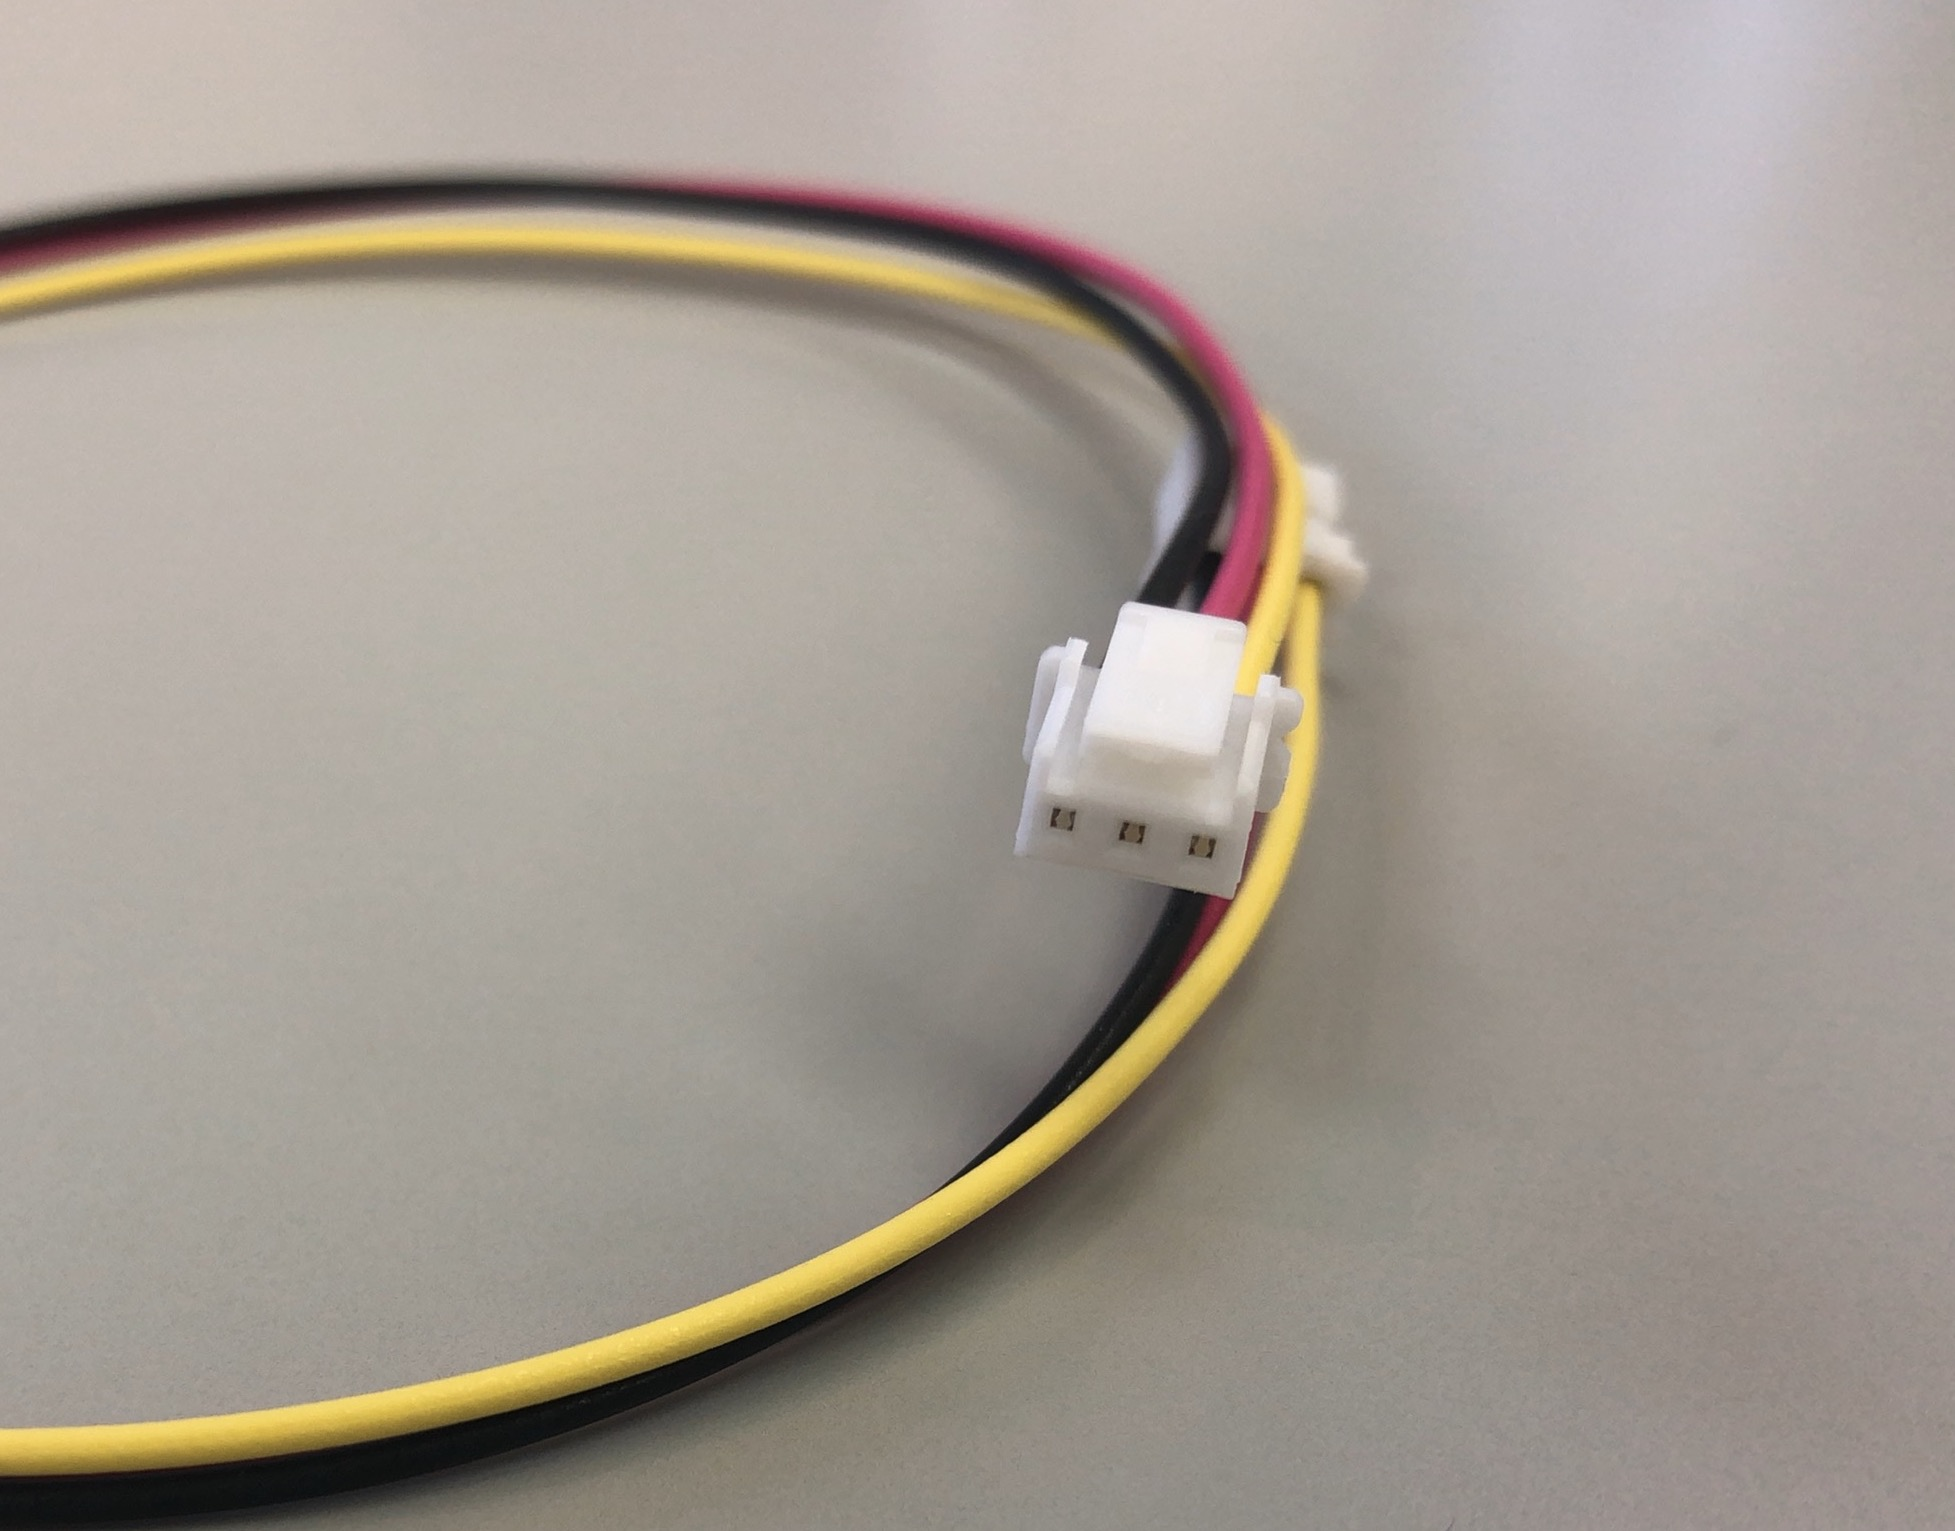
\includegraphics[width=0.8\hsize]{images/chap05/text05-img015.jpg}
    \caption{3ピンケーブル}
  \end{minipage}
\end{figure}











